\chapter{Preliminaries Concepts}
\label{preliminariesconcepts}

\section{Computational Complexity}
The \textbf{computational complexity}, or \textbf{complexity}, of an algorithm is the amount of resources (time and memory) needed for solving it, and it is the minimum complexity of all possible implementations for solving that given algorithm, included also the unknown ones \cite{wikipediacomplexity} (\href{https://en.wikipedia.org/wiki/Computational_complexity}{Computational complexity, Wikipedia}).

The amount of needed resources for solving an algorithm varies with the size of the input \(n\). The computational complexity in general is a function \(n \rightarrow f(n)\), and it represents the worst case complexity or the average complexity over all the inputs of size \(n\).

When the kind of the complexity is not explicitly indicated, generally is meant to be the \textbf{time complexity}, which is different from computer to computer, and it is generally expressed as the number of elementary operations required to solve a given algorithm. It is assumed that these elementary operations take the same time for being solved. The computational complexity can be related also to the memory consumption.

\section{Big O Notation}
The \textbf{big O notation} \cite{wikipediabigo} (\href{https://en.wikipedia.org/wiki/Big_O_notation}{Big O Notation, Wikipedia}) describe the behavior of a function when its argument tents to infinity or to a particular value.

\begin{definition}
Let \(f\) be a real or complex value function and let \(g\) be a real function. Let both functions be defined on the same positive and real unbounded interval, and let \(g(x)\) be strictly positive for all large enough \(x\) values: \(g(x) > 0, \forall x\) large enough. Thus: \(f(x)=O(g(x)) \) as \(x \rightarrow \infty \) if \(\exists\) \(M \in \mathbb{R} \), \(M>0\) and \(x_{0} \in \mathbb{R} \) such that \(|f(x)| \leq Mg(x)\) \(\forall x \geq x_{0}\). 
\end{definition}
Usually \(f(x)=O(g(x))\) is used as \(x \rightarrow \infty\), but it can be also defined for the case \(x \rightarrow a\), where \(a\) is a real number.

\(O\) notation is asymptotic for big \(x\), so the important terms are the ones which grow faster than the others, which become irrelevant.

\begin{example}
In \(f(x) = 6x^{4} - 2x^{3} + 5\) as \(x \rightarrow \infty\), \(6x^{4}\) it the fastest growing term. \(6\) is a constant and can be omitted, thus \(f(x)=O(x^{4})\).  
\end{example}

\subsection{Properties}
Here are listed some simple properties about Big O notation.
\begin{definition}[Product-Sum-Multiplication by a constant]
\textbf{Product} \\
\(f_{1}=O(g_{1})\) and \(f_{2}=O(g_{2})\) \(\Rightarrow\) \(f_{1}f_{2}=O(g_{1}g_{2})\)
\\
\textbf{Sum} \\
\(f_{1}=O(g_{1})\) and \(f_{2}=O(g_{2})\) \(\Rightarrow\) \(f_{1}f_{2}=O(max(f_{1}, f_{2}))\)
\\
\textbf{Multiplication by a constant} \\
Let \(k\) be a nonzero constant, then: 
\(O(k|g)=O(g)\), \(f=O(g)\) \(\Rightarrow\)\(kf=O(g)\)
\end{definition}

\begin{definition}[Logarithm and Exponential]
Let \(c\) be a nonzero constant, then: \(O(\log n^{c}) = O(\log n)\), because: (\(\log n^{c} = c \log n\)).
\\
\(O(n^{c})\) and \(O(c^{n})\) are very different, if \(c>1\) the latter grows much faster.
\\
Let \(c\) be a nonzero constant. \((cn)^{2}=c^{2}n^{2} = O(n^{2})\), but \(2^{n}\) and \(3^{n}\) are not of the same order. In general \(2^{cn}=(2^{c})^{n}\) is not of the same order of \(2^{n}\).
\end{definition}

\begin{example}
\(f = 9 \log n + 5(\log n)^{4} + 3n^{2} + 2n^{2} = O(n^{3})\) as \(n \rightarrow \infty\)
\end{example}

\begin{figure}[hb]
	\begin{center}
		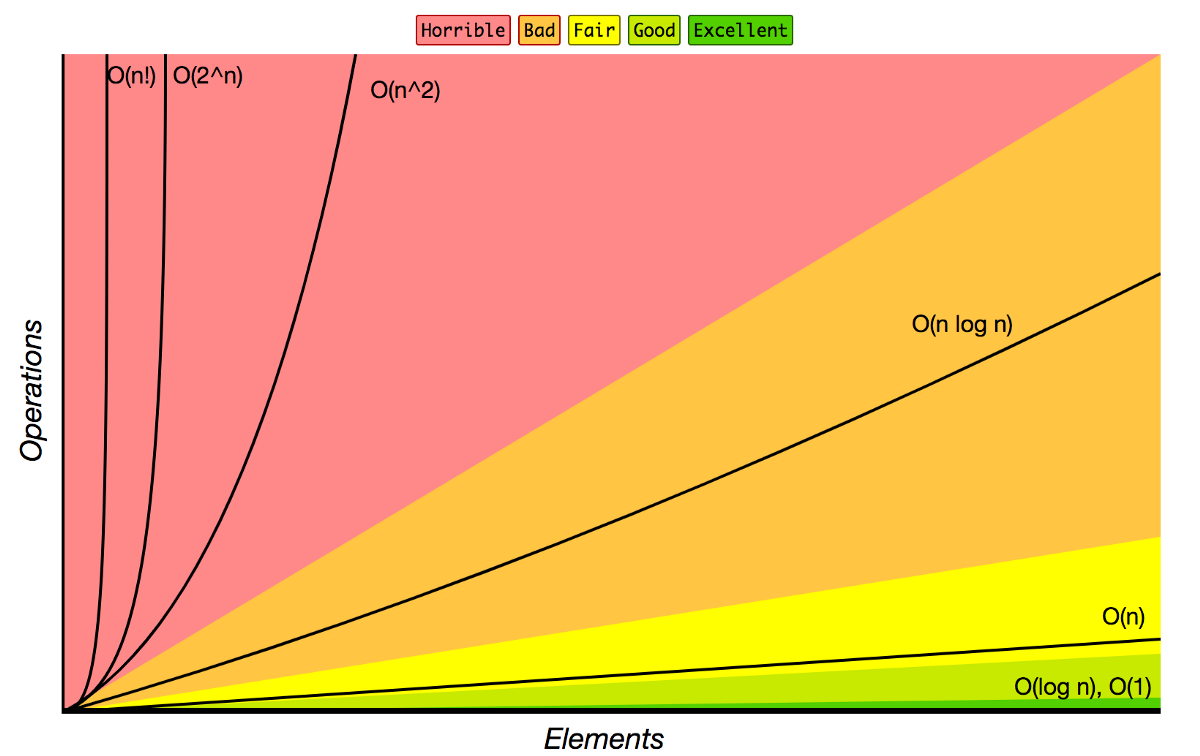
\includegraphics[scale=0.3]{chapters/introduction/images/big_o_plots.png}
		\caption[Plots of the main functions and their evaluation for computational complexity.]{Plots of the main functions and their evaluation for computational complexity. Credits: \href{https://www.bigocheatsheet.com/}{bigocheatsheet.com}.}
		\label{fig:bigoplots}
	\end{center}
\end{figure}

\section{Time complexity evaluation example}
Let us suppose we want to calculate the sum of all elements of a \(n\times n\) matrix. For evaluating the time complexity of this function we have to identify all the elementary operations, and evaluating their complexity based on how many times they are repeated. Here is the pseudocode for the function that calculate the sum of a matrix.

\begin{lstlisting}[firstnumber=1, caption={Sum of all elements of a matrix.}]
def find_sum_2d(array_2d):
	totoal = 0 # -> O(1)
	for each row in array_2d: # -> repeated n times
		for each column in array_2d: # -> repeated n times
			total += array_2d[column][row] # -> O(1)
	return total # -> O(1)
\end{lstlisting}

The total time complexity is: 
\[T = O(1) + n^{2}O(1) + O(1) = O(n^{2}) \]
Where \(O(1)\) is a constant value.

\section{Recursion}
In recursion a function calls itself again on a smaller size input, until the exit condition stops this self calling (recursive calling) \cite{wikirecursion} (\href{https://en.wikipedia.org/wiki/Recursion_(computer_science)}{Recursion, Wikipedia}). There are three fundamentals elements in a recursive function:
\begin{itemize}
\item[1] A function that calls itself.
\item[2] Exit condition. Without this condition a recursive function would call itself forever without an end.
\item[3] Input alteration. When the function is called again the input is changed to a smaller dimension than the previous call.
\end{itemize}

\begin{lstlisting}[numbers=none, caption={Pseudocode of a recursive function and its internal execution.}]
function recursive(input):
	if exit condition: # Element 2
		return input
	else:
		output = recursive(input-1) # Element 1
		return output # Element 3
\end{lstlisting}

In recursion the exit condition is fundamental, because if it contains some errors the recursion will never end, resulting in an infinite process.

\subsection{Python Implementation Examples}

\begin{lstlisting}[firstnumber=1, caption={Implementation of the Fibonacci series with both iterative and recursive way.}]
def fibonacci_iterative(position):
	if position == 0:
		return 0
	elif position == 1:
		return 1
	else:
		first = 0
		second = 1
		next_value = first + second
		for i in range(2, position):
			first = second
			second = next
			next_value = first + second
		return next_value

def fibonacci_recursive(position):
	if position <= 1: # Exit condition
		return position
	return fibonacci(position - 1) + fibonacci(position - 2) # Calling the function on a smaller size input
\end{lstlisting}

\begin{lstlisting}[firstnumber=1, caption={Implementation of calculating the factorial of a number using the recursive way.}]
def factorial(n):
	if n <= 1: # Exit condition
		return n
	else: 
		return n*factorial(n - 1) # Calling the function on a smaller input
\end{lstlisting}

\begin{figure}[H]
\centering
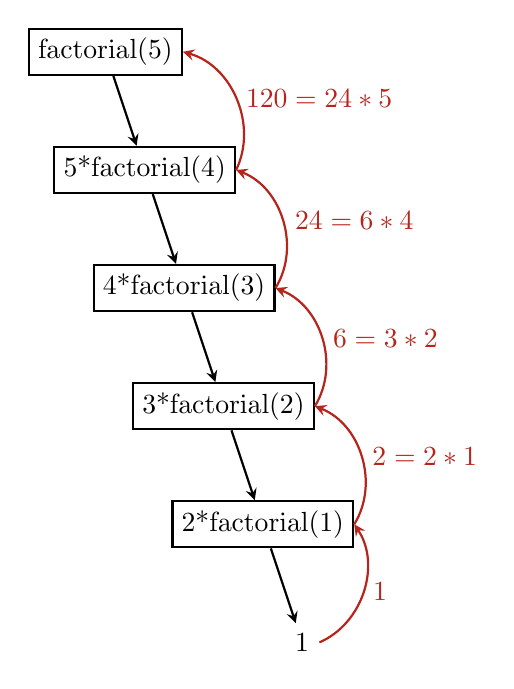
\begin{tikzpicture}[every node/.style={rectangle,draw}, node distance=15mm, thick]

	\node (n1) at (0,0) {factorial($5$)};
	\node (n2) at (0.5,-1.5) {$5$*factorial($4$)}; 
	\node (n3) at (1,-3) {$4$*factorial($3$)};
	\node (n4) at (1.5,-4.5) {$3$*factorial($2$)}; 
	\node (n5) at (2,-6) {$2$*factorial($1$)};
	\node[draw=none] (n6) at (2.5,-7.5) {$1$};

	\draw[->, >=stealth] (n1) -- (n2);
	\draw[->, >=stealth] (n2) -- (n3);
	\draw[->, >=stealth] (n3) -- (n4);
	\draw[->, >=stealth] (n4) -- (n5);
	\draw[->, >=stealth] (n5) -- (n6);
	
	\path[->, >=stealth, BrickRed] (n6.east) edge [bend right=50] node[draw=none, xshift=6pt] {$1$} (n5.east);
	\path[->, >=stealth, BrickRed] (n5.east) edge [bend right=50] node[draw=none, xshift=23pt] {$2=2*1$} (n4.east);
	\path[->, >=stealth, BrickRed] (n4.east) edge [bend right=50] node[draw=none, xshift=23pt] {$6=3*2$} (n3.east);
	\path[->, >=stealth, BrickRed] (n3.east) edge [bend right=50] node[draw=none, xshift=26pt] {$24=6*4$} (n2.east);
	\path[->, >=stealth, BrickRed] (n2.east) edge [bend right=50] node[draw=none, xshift=30pt] {$120=24*5$} (n1.east);

\end{tikzpicture}
\caption[Factorial recursive execution.]{Factorial recursive execution.}
\label{fig:factorial_1}
\end{figure}